%%%%%%%%%%%%%%%%%%%%%%%%%%%%%%%%%%%%%%%%%
% Dreuw & Deselaer's Poster
% LaTeX Template
% Version 1.0 (11/04/13)
%
% Created by:
% Philippe Dreuw and Thomas Deselaers
% http://www-i6.informatik.rwth-aachen.de/~dreuw/latexbeamerposter.php
%
% This template has been downloaded from:
% http://www.LaTeXTemplates.com
%
% License:
% CC BY-NC-SA 3.0 (http://creativecommons.org/licenses/by-nc-sa/3.0/)
%
%%%%%%%%%%%%%%%%%%%%%%%%%%%%%%%%%%%%%%%%%

%----------------------------------------------------------------------------------------
%	PACKAGES AND OTHER DOCUMENT CONFIGURATIONS
%----------------------------------------------------------------------------------------

\documentclass[final,hyperref={pdfpagelabels=false},12pt]{beamer}

\usepackage[orientation=portrait,size=a0,scale=1.3]{beamerposter} % Use the beamerposter package for laying out the poster with a portrait orientation and an a0 paper size

\usepackage[absolute,overlay]{textpos}


\usetheme{I6pd2} % Use the I6pd2 theme supplied with this template

\usepackage[english]{babel} % English language/hyphenation

\usepackage{amsmath,amsthm,amssymb,latexsym} % For including math equations, theorems, symbols, etc

%\usepackage{times}\usefonttheme{professionalfonts}  % Uncomment to use Times as the main font
%\usefonttheme[onlymath]{serif} % Uncomment to use a Serif font within math environments

\boldmath % Use bold for everything within the math environment

\usepackage{booktabs} % Top and bottom rules for tables

\graphicspath{{figures/}} % Location of the graphics files

\usecaptiontemplate{\small\structure{\insertcaptionname~\insertcaptionnumber: }\insertcaption} % A fix for figure numbering


\usepackage{ragged2e}    %% provides \justifying
\let\olditem\item
\renewcommand{\item}{\olditem\justifying}


\setbeamercolor*{thcolor}{fg=blue!60}

\makeatletter
\setbeamertemplate{theorem begin}
  {\usebeamercolor[fg]{thcolor}% for the heading
  {\bfseries\inserttheoremname~}%
  \ifx\inserttheoremaddition\@empty\else(\inserttheoremaddition)\ \fi%
  \hspace{.01em}\normalfont\usebeamercolor[fg]{thcolor}% for the body
  }
\setbeamertemplate{theorem end}{}
\makeatother


%% Define a HUGE 
\usepackage{fix-cm}    

\usepackage{caption}
\usepackage{graphicx}

\makeatletter
\newcommand\HUGE{\@setfontsize\Huge{112}{50}}
\makeatother    


\let\Tiny\tiny% http://tex.stackexchange.com/q/58087/5764
\usepackage{xparse}
\makeatletter
\NewDocumentCommand{\figcaption}{s o m}{%
  \par\IfBooleanF{#1}{\refstepcounter{figure}}% Step figure counter
  {\footnotesize\IfBooleanF{#1}{\alert{Figure~\thefigure}: }#3\par}%
  \xdef\@currentlabelname{\IfNoValueTF{#2}{#3}{#2}}%
}
\makeatother
%----------------------------------------------------------------------------------------
%	TITLE SECTION 
%----------------------------------------------------------------------------------------

\title{\HUGE  MAA--FTYCMA JOINT CONFERENCES} % Poster title

\author{Joni Pirnot, C. Altay \"Ozgener, Local Organization Chairs} 
% Author(s)

%\begin{center}


\institute{State College of Florida, Manatee--Sarasota, Bradenton, FL}
%\end{center}
% Institution(s)

%----------------------------------------------------------------------------------------
%	FOOTER TEXT
%----------------------------------------------------------------------------------------

\newcommand{\leftfoot}{http://sections.maa.org/florida/ \& http://scf1.scf.edu/ftycma/default.htm} % Left footer text

\newcommand{\rightfoot}{MAA-FTYCMA JOINT CONFERENCES 2017} % Right footer text

%----------------------------------------------------------------------------------------

\begin{document}

\addtobeamertemplate{block end}{}{\vspace*{2ex}} % White space under blocks

\begin{frame}[t] % The whole poster is enclosed in one beamer frame

\begin{columns}[t] % The whole poster consists of two major columns, each of which can be subdivided further with another \begin{columns} block - the [t] argument aligns each column's content to the top

\begin{column}{.02\textwidth}\end{column} % Empty spacer column

\begin{column}{.465\textwidth} % The first column

%----------------------------------------------------------------------------------------
%	OBJECTIVES
%----------------------------------------------------------------------------------------

\begin{block}{Call for Presentations}

The annual joint meetings of the MAA-Florida Section and FTYCMA will be held on {\bf {February 17-18, 2017}} on the campus of \href{http://www.scf.edu/}{State College of Florida}.  We invite talks (either $20$ minutes or $45$ minutes in duration) and workshops or special topic sessions ($105$ minutes) from mathematicians in the State University System, the Florida Community College System, and the state's private colleges and universities. Graduate and undergraduate students are also invited to participate. 




\end{block}

%----------------------------------------------------------------------------------------
%	INTRODUCTION
%----------------------------------------------------------------------------------------
            
\begin{block}{Proposals}

Those who wish to be considered for the program talks or workshops should send their name, institutional affiliation, title, and an abstract of one hundred and fifty words or less to the Florida Section's Vice-President for Programs, 
\href{mailto:djelsovsky@flsouthern.edu?subject=FL-MAA Call for Papers 2017}{Daniel Jelsovsky}, and indicate a talk or workshop and its duration.  This information should be sent via e-mail as a Word document.  Deadline for submission is \bf{December 16, 2016}.


\end{block}

%----------------------------------------------------------------------------------------
%	MATERIALS
%----------------------------------------------------------------------------------------

\begin{block}{Talks}

Talks will be in \textcolor{blue}{Building \# 9} (close to \textcolor{blue}{lot J}, and at State College of Florida's \textcolor{green}{Neel Performing Arts Center} (Building \# 11), (see \href{cmap.jpg}{Campus map}). 

\end{block}

%----------------------------------------------------------------------------------------
%	METHODS
%----------------------------------------------------------------------------------------

\begin{block}{Forms}

Here are the forms in PDF and Word formats.

\begin{itemize}

\item Pre-registration Forms (Faculty)
    \begin{itemize}
\item \href{preregistration_f.pdf}{PDF}    
\item \href{preregistration_f.docx}{Word} 
    \end{itemize}           
                        
\item Student Preregistration Form (Student)
    \begin{itemize}
\item \href{preregistration_s.pdf}{PDF} 
\item \href{preregistration_s.docx}{Word} 
   \end{itemize}


\end{itemize}



\end{block}

%----------------------------------------------------------------------------------------
%	MATHEMATICAL SECTION
%----------------------------------------------------------------------------------------
%\begin{center}
\begin{block}{Conference Program}

%\begin{center}
\begin{itemize}
\item {\bf Program} \href{program.pdf}{PDF} 
\item {\bf  Plenary Speakers} \href{ps.htm}{Plenary Speakers} 
\item {\bf Directions}
\href{http://www.scf.edu/AboutSCF/Locations/SCFBradenton/default.asp}
				{Directions to State College of Florida, Bradenton Campus}
\item {\bf Parking}
Parking on Campus, use \textcolor{blue}{lot J}  (see  \href{cmap.jpg}{Campus map})
\end{itemize}

%\end{center}
\end{block}
%\end{center}

\begin{block}{Accommodations}


For the hotels listed below, ask for {\bf the State College of Florida February Math Conference discount}. Quoted rates are subject to availability.
\begin{itemize}
\item \href{http://www.marriott.com/hotels/travel/srqcy-courtyard-sarasota-bradenton-airport/}{Courtyard Sarasota Bradenton Airport}\\
 850 University Parkway\\
 Sarasota  Florida  34234\\
$941\cdot 355\cdot3337$\\
Details: Double \$239.00.  Group code {\sc SMERF}.  Deadline 1/26/2017.
\item \href{http://tinyurl.com/CIS-MAA-FTYCMA}{Country Inn \& Suites Bradenton}\\
5610 Manor Hill Lane\\
 Bradenton, FL 34203\\
 $941\cdot 363\cdot 4000$ or $800\cdot 456\cdot 4000$ \\
 Details:  Complimentary full American hot breakfast buffet, free high speed Internet. \\
Queen/Queen guestrooms  \$169                         
 	King Guestroom   \$169                                            
 	King Studio with Sofa pullout   \$179                       
 	One bedroom King Suite with sofa pullout   
 	\$189.\\          
 Group code {\sc FTYCMA}.Deadline 1/26/2017.
\item \href{https://www.holidayinn.com/redirect?path=hd&brandCode=hi&localeCode=en&regionCode=1&hotelCode=SRQAP&_PMID=99801505&GPC=MAA&viewfullsite=true }{Holiday Inn Sarasota Bradenton}\\
8009 15th Street East\\
 Sarasota, FL 34243\\
{\bf  800-HOLIDAY}  \\
 Details: {\sc MAA/FTYCMA Conference}

\end{itemize}
\end{block}


\begin{block}{Menu}

{\bf Banquet Menu} \\
 Poached Salmon\\ 
 Chicken Champagne\\
 Wild Mushroom Ravioli\\ 
 Steamed Baby Redskin Potatoes with Parsley Butter,
 Green Beans Almandine\\ 
 Chocolate Sheet Cake  \\

{\bf Lunch Menu}\\
 Pasta Primavera\\
 Meat \& $3$ Cheese Lasagna
\end{block}
%----------------------------------------------------------------------------------------

\end{column} % End of the first column



\begin{column}{.03\textwidth}\end{column} % Empty spacer column
 
\begin{column}{.465\textwidth} % The second column

%----------------------------------------------------------------------------------------
%	RESULTS
%----------------------------------------------------------------------------------------

\begin{block}{Plenary Speakers}

\begin{itemize}
\item Tim Chartier – VP, MAA\\

{\emph{March Mathness}}

Every year, people across the United States predict who will win in the Division I NCAA Men's Basketball Tournament, often called March Madness, by filling out a tournament bracket for the postseason play. This talk discusses two popular rating methods that were used by the Bowl Championship Series, the organization that determined which college football teams were invited to which bowl games. Each rating method computes a ranking by solving a system of linear equations. We also touch on how to adapt the methods to take late season momentum into account. By the end, you'll be ready to create a mathematically-produced bracket for March Madness.


\item Ken Ono – Emory University\\

{\emph{Gems of Ramanujan and their Lasting Impact on Mathematics}}

Ramanujan's work has a truly transformative effect on modern mathematics, and continues to do so as we understand further lines from his letters and notebooks. In this lecture, some of the studies of Ramanujan that are most accessible to the general public will be presented and how Ramanujan's findings fundamentally changed modern mathematics, and also influenced the lecturer's work, will be discussed. The speaker is an Associate Producer of the film The Man Who Knew Infinity (starring Dev Patel and Jeremy Irons) about Ramanujan. He will share several clips from the film in the lecture.

\end{itemize}     
\end{block}

%------------------------------------------------

\begin{block}{Plenary Speakers}


\begin{figure}[ht]
        \begin{minipage}[b]{0.45\linewidth}
            \centering
            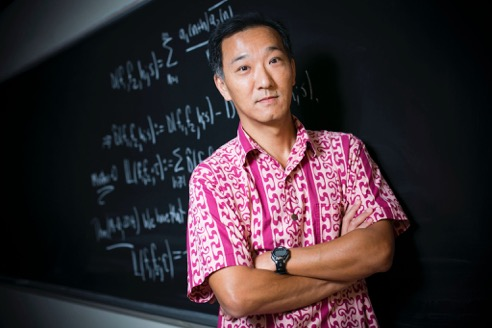
\includegraphics[width=\textwidth]{ken}
            \figcaption*{Ken Ono}
            \label{fig:a}
        \end{minipage}
        \hspace{0.5cm}
        \begin{minipage}[b]{0.45\linewidth}
            \centering
            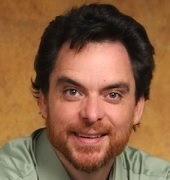
\includegraphics[scale=.35,width=\textwidth]{tim}
            \figcaption*{Tim Chartier}
            \label{fig:b}
        \end{minipage}
    \end{figure}

\end{block}

%----------------------------------------------------------------------------------------
%	CONCLUSION
%----------------------------------------------------------------------------------------

\begin{block}{``BY THE NUMBERS''}
{\emph{BY THE NUMBERS}} is a series of short plays commissioned by the SCF theatre and math departments. Four award-winning professional theatre artists based in New York City, none of whom are mathematically talented and all of whom struggle to balance their checkbooks, allow themselves to be inspired by the names of famous theorems. Exploring the intersection between science and art by reading about math and talking to mathematicians, the playwrights' imaginations take flight, creating, for the SCF theatre students to decipher and perform, a cycle of dark, funny universes.


\end{block}

%----------------------------------------------------------------------------------------
%	REFERENCES
%----------------------------------------------------------------------------------------

\begin{block}{Aftermath}
        
The Fine Art Gallery at the State College of Florida will host a reception from 8-10 PM on Friday, February 17, for its newest exhibit, ``Richard Anuszkiewicz: Inward Eye.'' The exhibit includes the words of the poet 	and painter William Blake and was chosen to emphasize the relationship of mathematics to the fine arts. 	Skillfully planned and executed, Anuszkiewicz's images allow him to focus on color and geometry; combined 	with Blake's words, the images produce associations that can transform meaning.

\end{block}

%----------------------------------------------------------------------------------------
%	ACKNOWLEDGEMENTS
%----------------------------------------------------------------------------------------

\begin{block}{Acknowledgments}

We would like to thank Pearson, CENGAGE, WebAssign, Hawkes Learning.

State College of Florida  and its president Carol F. Probstfeld  
 generously provided some funding for the conference.


\end{block}

%----------------------------------------------------------------------------------------
%	CONTACT INFORMATION
%----------------------------------------------------------------------------------------

\setbeamercolor{block title}{fg=black,bg=orange!70} % Change the block title color

\begin{block}{Websites and Contact Information}

 \begin{minipage}[b]{0.45\linewidth}
 \begin{itemize}
\item  \href{http://sections.maa.org/florida/}{MAA-FL}
\item  \href{http://scf1.scf.edu/ftycma/default.htm}{FTYCMA}
\item \href{http://www.scf.edu/}{SCF}
\item  \href{http://www.scf.edu/Academics/FinePerformingArts/FineArtGallery/default.asp}{Fine Arts Gallery}
\end{itemize}
        \end{minipage}
        \hspace{0.5cm}
        \begin{minipage}[b]{0.45\linewidth}
       \begin{itemize}
\item Phone: $941\cdot 752\cdot 5224$
\item Local Organization Chairs:\\  Joni Pirnot \& C. Altay \"Ozgener 
\end{itemize}
        \end{minipage}



\end{block}

%----------------------------------------------------------------------------------------

\end{column} % End of the second column

\begin{column}{.015\textwidth}\end{column} % Empty spacer column

\end{columns} % End of all the columns in the poster

\end{frame} % End of the enclosing frame

\end{document}
